\documentclass[12pt]{article}
\usepackage[spanish]{babel}
\usepackage{lingmacros}
\usepackage{tree-dvips}
\usepackage{amsmath, amsthm, amssymb}
\usepackage{graphicx}
\begin{document}


\title{Car accidents on Seattle, a view of data}

\author{Carlos Ríos} 
\date{\small{\today}}

\maketitle


\section*{}
\subsection*{Why? (Introduction)}
This work is aimed at society in general and the objective is to generate social awareness regarding traffic accidents, for that reason the language will be simple. Taking into account that traffic accidents represent the death of 1.3 million people around the world each year (*World Health Organization*, link https://www.who.int/features/factfiles/roadsafety/es/), in this This work aims to better understand this type of accident, and evaluate which are the most relevant factors for their occurrence. According to the *World Health Organization*, victims (worldwide) correspond to passersby in 50\% of cases, it is also explained that most accidents in general occur due to human errors, however there are also environmental factors, automobile, or the roads. Mainly we are going to use Machine Learning to create a model that classifies accidents according to their level of severity in order to predict the probability of an accident according to new features.
 \

\begin{figure}[htbp]
  \centering
    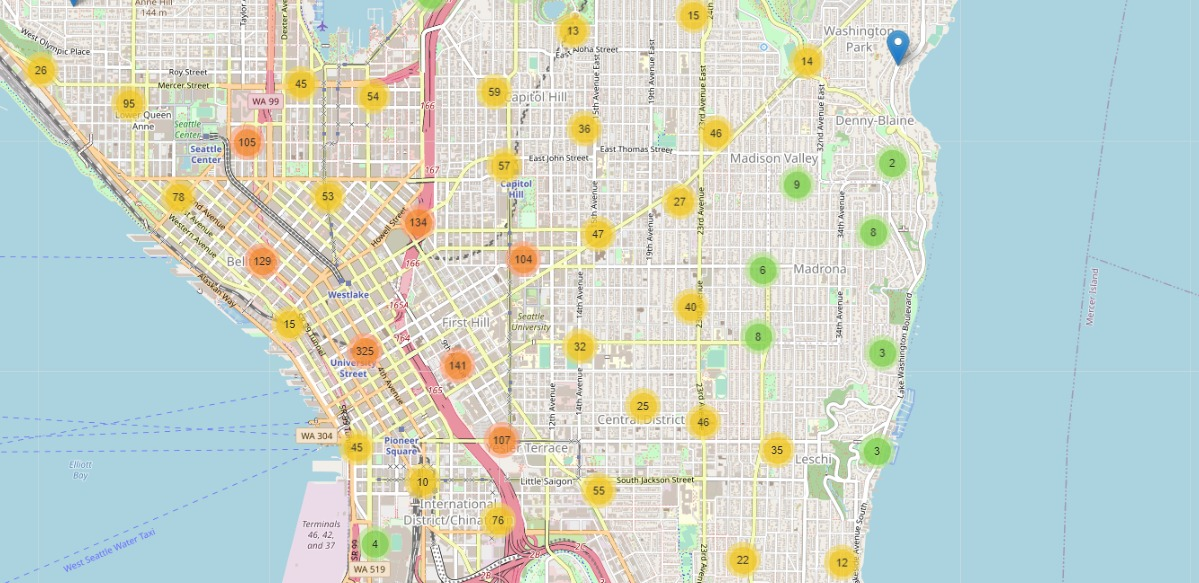
\includegraphics[width=1\textwidth]{../images/map_d.jpeg}
  \caption{Gráfico del ejercicio, el punto P esta en algun lugar entre P1 y P2}
  \label{fig:ejemplo}
\end{figure}

 
\begin{equation}
  r=\frac{P_{1}P}{PP_{2}}=\frac{\sqrt{(x-x_{1})^{2}+(y-y_{1})^{2}}}{\sqrt{(x_{2}-x)^{2}+(y_{2}-y)^{2}}}
  \label{eq:razon}
  \end{equation}
  \begin{figure}[htbp]
    \centering
      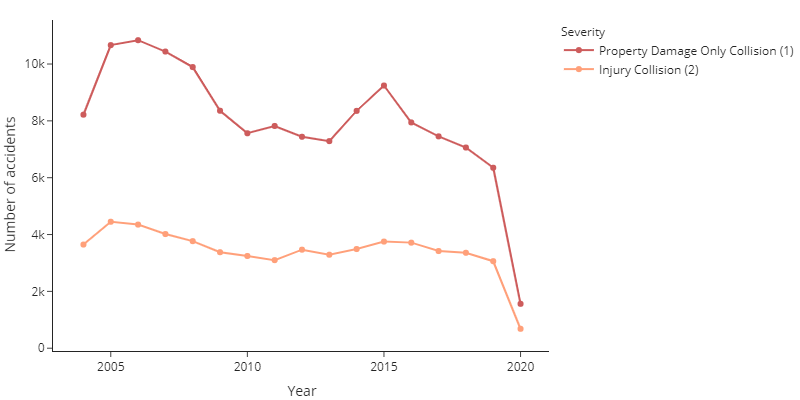
\includegraphics[width=1\textwidth]{../images/years.png}
    \caption{Gráfico del ejercicio, el punto P esta en algun lugar entre P1 y P2}
    \label{fig:ejemplo}
  \end{figure}


\subsection*{About the data}
I will use the *Collisions database - Every year* provided by the *Seattle SDOT Traffic Management Division*. The data is made up of 194673 cases, and contains 38 characteristics which I will separate into four groups:

**a)** There are some **characteristics that are not relevant** for our purpose, for example those that correspond to identification codes (id), there are also repeated characteristics or characteristics with little information.

**b)** There are **features that may not be relevant to apply machine learning techniques but that are relevant to better understand the problem**, for example the location and coordinates.

**c)** Finally there are **features that I don't know if they will really be useful to me**.

**d)** On the other hand, there are those **characteristics that probably have a strong influence on the severity** of the accident. Even these have to be worked on because many contain a numerical code that does not refer to a numerical value but is an identification code for a certain type of accident.



Next I will make an explanation of each of these groups.

\begin{figure}[htbp]
    \centering
      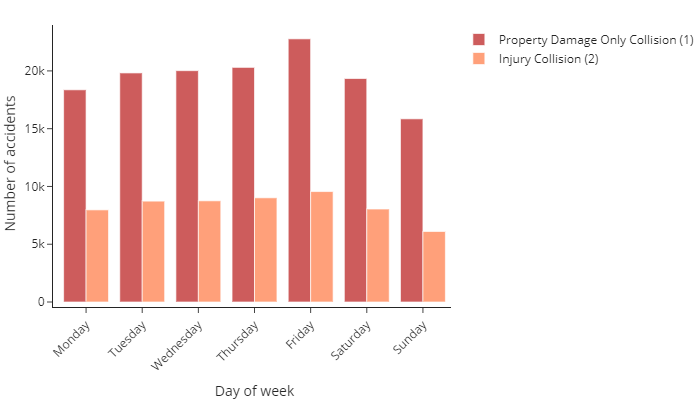
\includegraphics[width=1\textwidth]{../images/day_of_week.png}
    \caption{Gráfico del ejercicio, el punto P esta en algun lugar entre P1 y P2}
    \label{fig:ejemplo}
  \end{figure}
Comenzamos analizando cuando deberia se el valor de r. Sabemos que la distancia $P_{1}P=2PP_{2}$, donde P es el punto intermedio.
Entonces
\begin{equation}
  \frac{P_{1}P}{PP_{2}}=2=r
  \label{r}
  \end{equation}

  \begin{figure}[htbp]
    \centering
      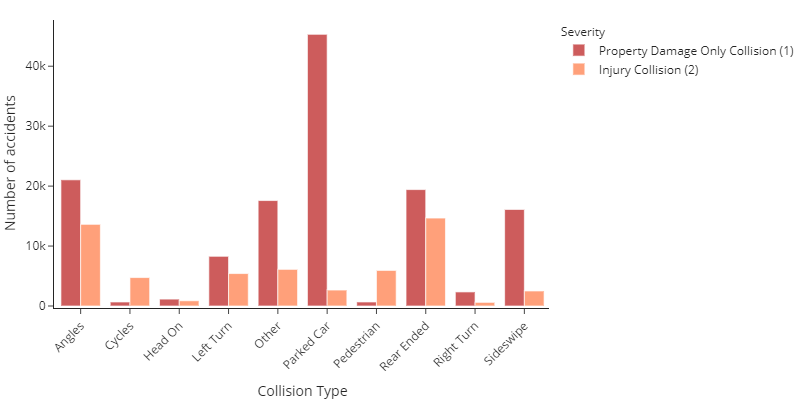
\includegraphics[width=1\textwidth]{../images/collition_type.png}
    \caption{Gráfico del ejercicio, el punto P esta en algun lugar entre P1 y P2}
    \label{fig:ejemplo}
  \end{figure}

\end{document}